\section{Routing-Atlas}\label{sec:routingatlas}

Der Routing-Atlas ist ein Projekt der FU Berlin und der HAW Hamburg in Zusammenarbeit mit dem Bundesamt für Sicherheit in der Informationstechnik (BSI), \vgl \cite{wsbh-envgi-12}.
Das Projekt will landesspezifische Bestandteile des Internets identifizieren, klassifizieren und visualisieren.
Diese Daten sollen vielfältige Fragestellungen beantworten helfen.
Zum Beispiel nach der Abhängigkeit der Länder untereinander, nach der Abgeschlossenheit der Infrastruktur innerhalb eines Landes und nach der Bedeutung einzelner Akteure.

Erster Schritt des Projektes ist es eine möglichst korrekte Zuordnung von Bestandteilen des Internets zu Ländern durchzuführen.
Als Beispiel dient hierbei Deutschland.
Gegenüber vorherigen Arbeiten zum Beispiel von Josh Karlin et~al.~\cite{0903.3218v1} wird die Zuordnung nicht ausgehend von IP-Präfixen sondern feingranularer auf Ebene von IP-Adressblöcken vorgenommen.
Die Zuordnung der IP-Adressblöcke zu einem Land geschieht basierend auf Daten der zuständigen RIR - für Deutschland die RIPE~\cite{RIPE} - in einem mehrstufigen Verfahren.
Als Kandidaten werden jene Adressblöcke betrachtet, deren \texttt{country} Attribut "`DE"' oder "`EU"' lautet.
Zu Verfizierung der "`DE"' und zur Identifizierung weiterer "`EU"' als deutsch werden nun Kontaktinformationen zu den Adressblöcken ausgewertet und gegen eine Liste von Synonymen, geographischen Namen und Schlagworten abgeglichen.
Die so als deutsch identifizierten Adressblöcke werden nun zu IP-Präfixen und anschließend zu ASen aufgelöst.

Die einem Land zugehörigen ASe werden nach den Aspekten Hierarchie und Branche klassifiziert.
Die Hierarchie gibt an, welche Bedeutung ein AS für das Routing hat und wird aus Daten von Beichuan Zhang et~al.~\cite{Zhang:2005:CIA:1052812.1052825} übernommen.
Die Branche ordnet ein AS einem der folgenden Sektoren zu:
\begin{center}
  \begin{tabular}[h]{ll}
    \hline
    Behören, Verwaltung und Justiz & I\&K: Software- und Systeme \\
    Energie & Industrie (Produzierendes Gewerbe) \\
    Finanz-, Geld- und Versicherungswesen & Medizinwesen \\
    Gefahrenstoffe & Presse, Medien, Verlage \\
    I\&K: Internet Peering Points & Transport und Verkehr \\
    I\&K: ISPs (ohne Endkunden-Zugang),\\
    Internet Infrastruktur & Wissenschaft, Forschung \& Kultur \\
    I\&K: Access Provider & Sonstiges \\
    \hline
  \end{tabular}
\end{center}
Die Branchenzuordnung geschieht basierend auf einer Liste von Schlagworten, die mit den in der RIPE DB vorhandenen Metainformationen (Name, Beschreibung und Adressfeldern) der ASen verglichen wird.

Für die identifizierten und klassifizierten ASe wird der umspannende Routing-Graph durch Traversieren der verbindenden Pfade zwischen allen Paaren der als deutsch identifizierten ASe ermittelt.
Dazu wird die shortest path matrix von Winter (\vgl Abschnitt~\ref{subsec:winter}) genutzt.
Erwartungsgemäß werden damit bisher nicht betrachtete verbindende ASe anderer Länder aufgenommen.

Der so entstandene, mit den Eigenschaften Land, Hierarchie und Sektor annotierte Graph wird anschließend visualisiert.
Um dabei Aussagekraft und Übersichtlichkeit zu steigern, wird der Graph nach unterschiedlichen Aspekten vorgefiltert und auf verschiedene Arten visualisiert.
So werden zum Beispiel die ASe zweier Sektoren gegenübergestellt und durch die verbindenden, nach Hierarchie angeordneten ASe ergänzt.
Weitere Darstellungen zeigen ASe eines Sektoren inklusive verbindender ASe wahlweise hierarchisch in Schichten oder Ringen angeordnet oder unsortiert.
Die Farbe der Knoten steht dabei für den Sektor des zugehörigen AS.
Abbildung~\ref{fig:asgraph_cat10} auf Seite~\pageref{fig:asgraph_cat10} zeigt die Autonomen Systeme des Sektors "`Wissenschaft, Forschung \& Kultur (F\&E)"' in einem hierarchischen Kreisdiagramm.
Die Position eines AS in diesem Diagramm bedeutet, dass es in seiner topologischen Bedeutung (von innen nach außen) Tier 1, Large ISP, Small ISP und Stub zuzuordnen ist.

\begin{figure}
  \begin{center}
  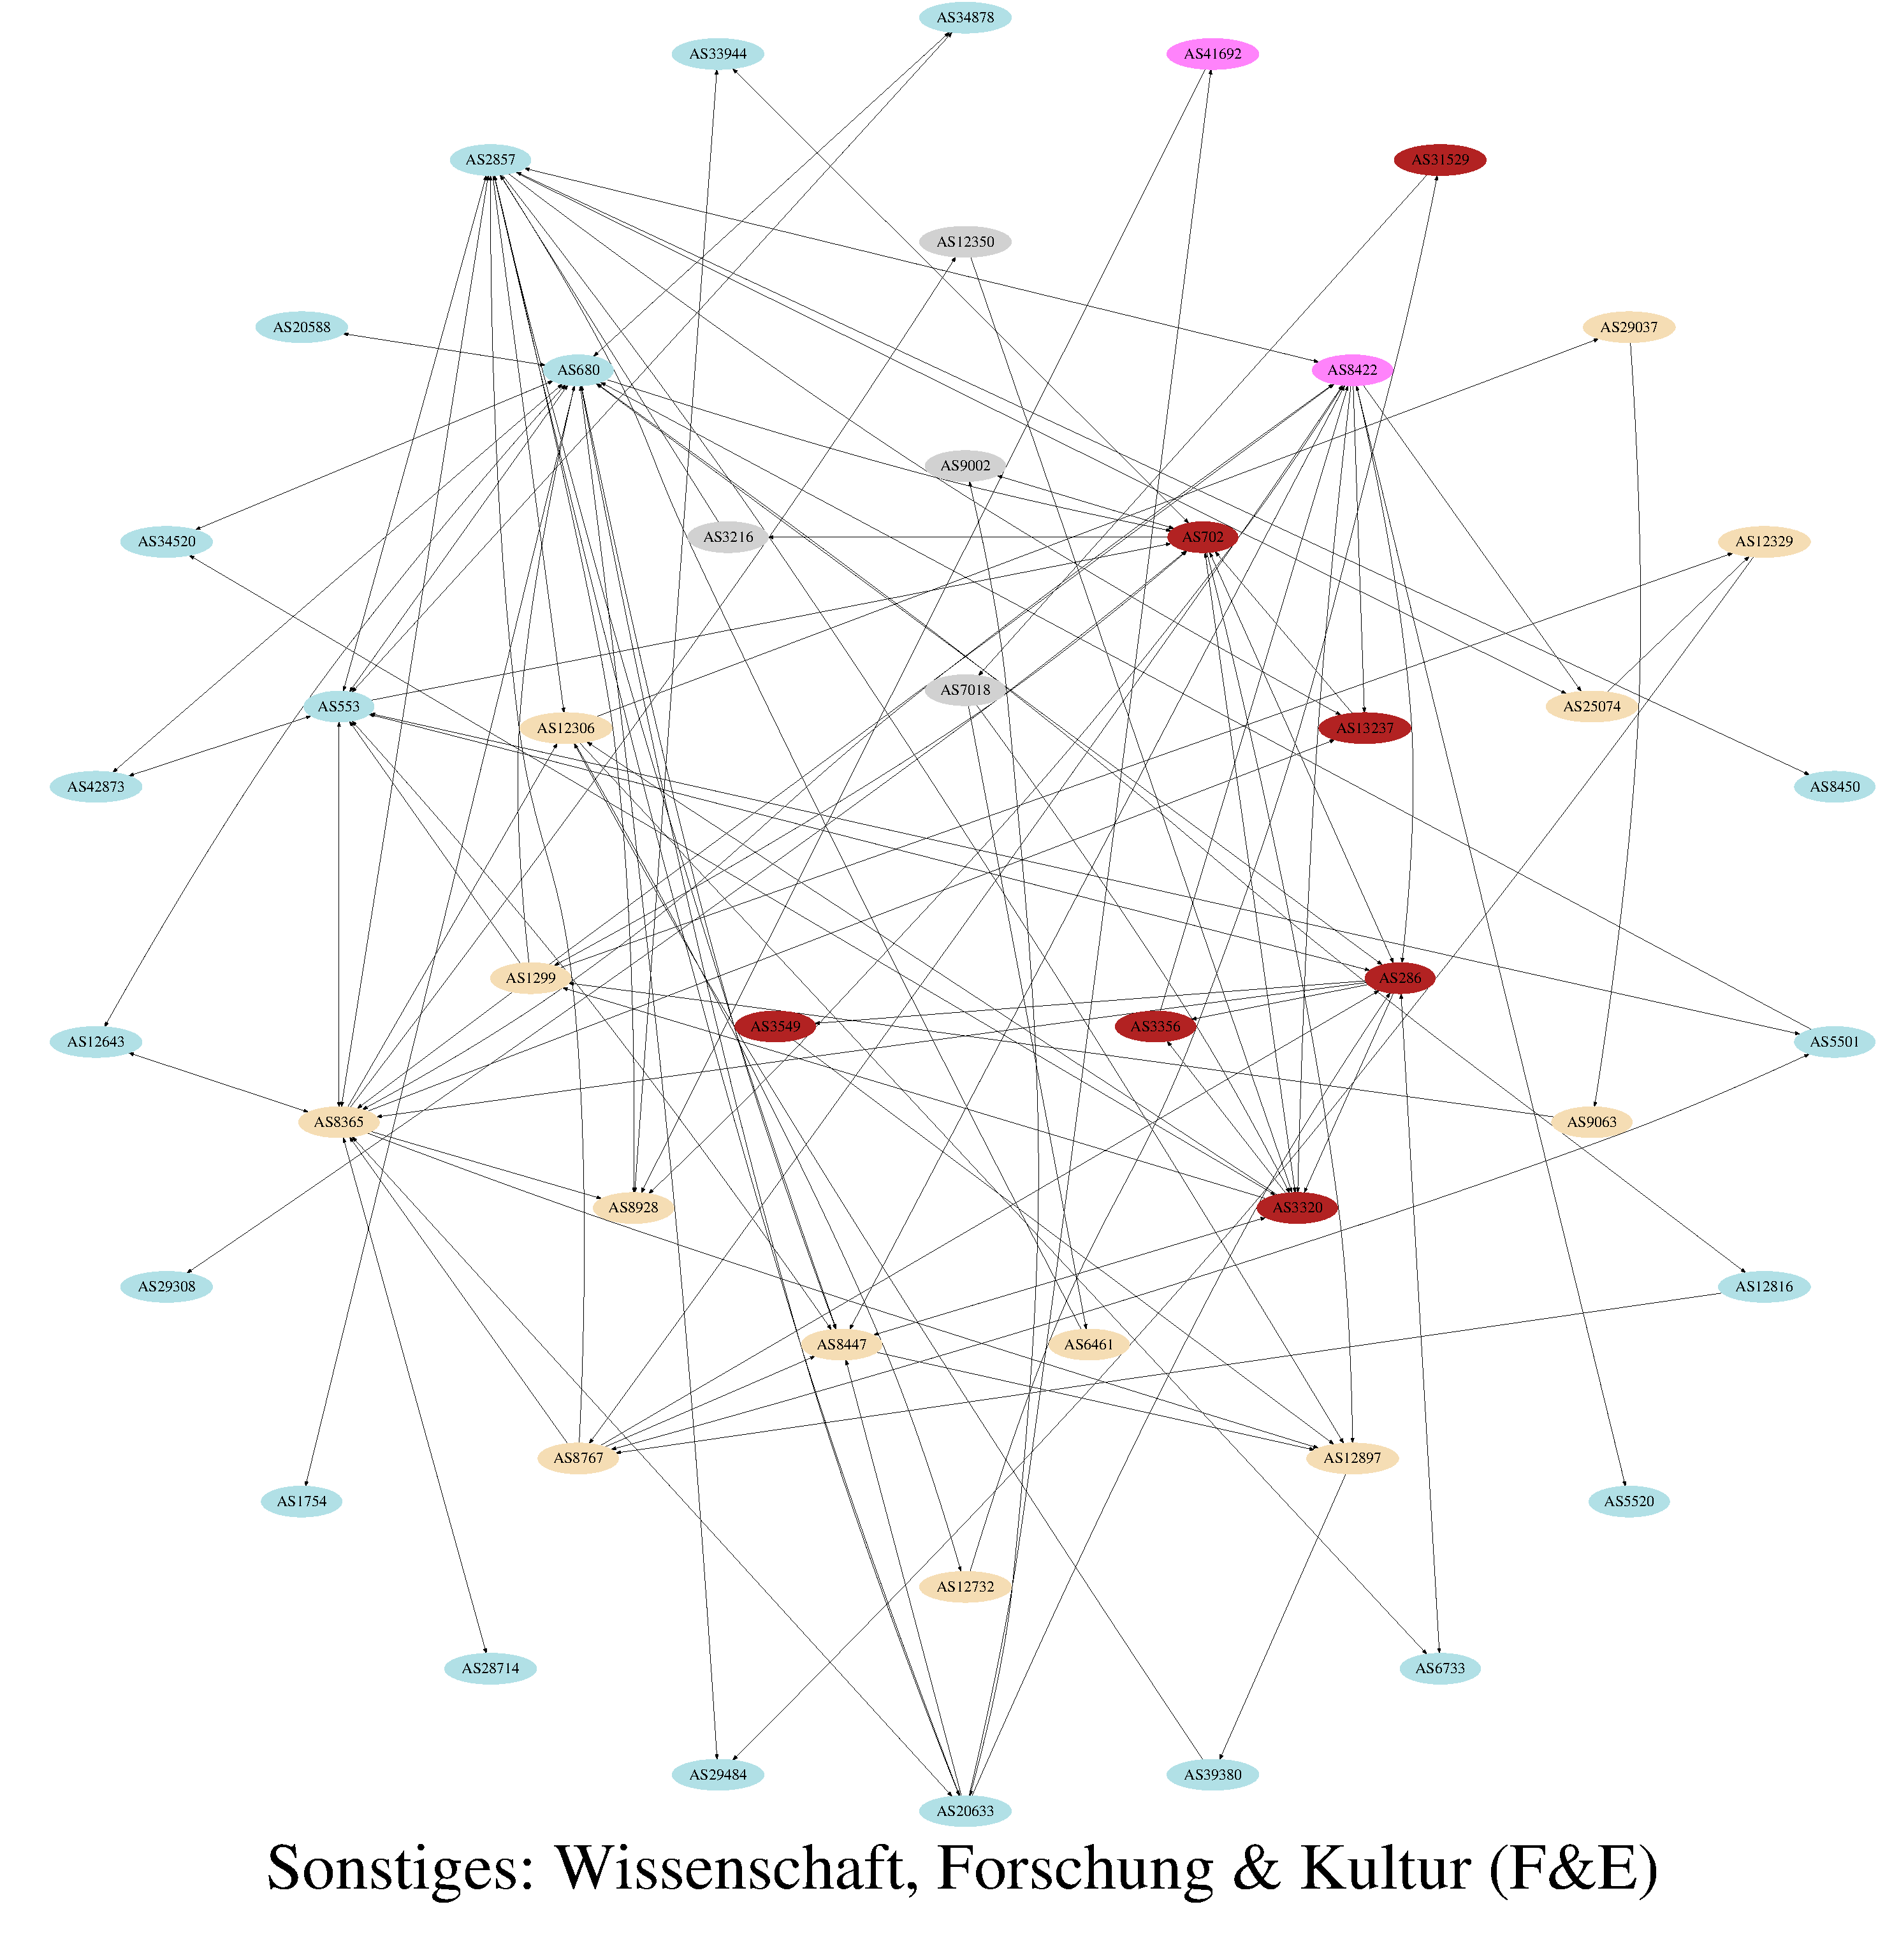
\includegraphics[width=0.55\textwidth]{asgraph_cat10-pos}
  \caption{Hierarchisches Kreismodell - Entnommen aus~\cite{swbh-rsved-11}} \label{fig:asgraph_cat10}
  \end{center}
\end{figure}
